\section{第VIポジション \label{6th}}

\begin{center}
\begin{tabular}{|lcl|}
\hline
この章の基礎練習 & : & 1. 開放弦の練習 2. 「\ref{5th_scale}」「\ref{2nd-3rd_scale}」「\ref{5th-6th_scale}」の音階練習 3. ドヴォルザーク\\
この章の修了課題 & : & 1. 「\ref{6th_scale}」の音階練習を正しい音程で暗譜して演奏できる\\
               &   & 2. ベルリオーズ、チャイコフスキー、ハイドンのいずれか1曲を暗譜\\
\hline
\end{tabular}
\end{center}

\begin{flushleft}
\begin{minipage}{260pt}
\subsection{第VIポジションの位置}
\ \ \ \ このポジションからは4の代わりに3の指を使います。さらに親指の位
置も変わります。既出のポジションではネックの裏にあった親指が、今度は指
板の横に置くようになります(図
\addtocounter{figure}{2}\thefigure\addtocounter{figure}{-2})。また、こ
のポジションの3の指は弦長\(\frac{1}{2}\)地点に位置していますので、開放
弦の1オクターヴ上のフラジオレット音が出ます。第VIポジションで取れる音は、
細い方の隣の弦の第IIIポジションの音に対応しています。
\end{minipage}
\hfill
\begin{minipage}{140pt}
\addtocounter{figure}{1}
\begin{center}
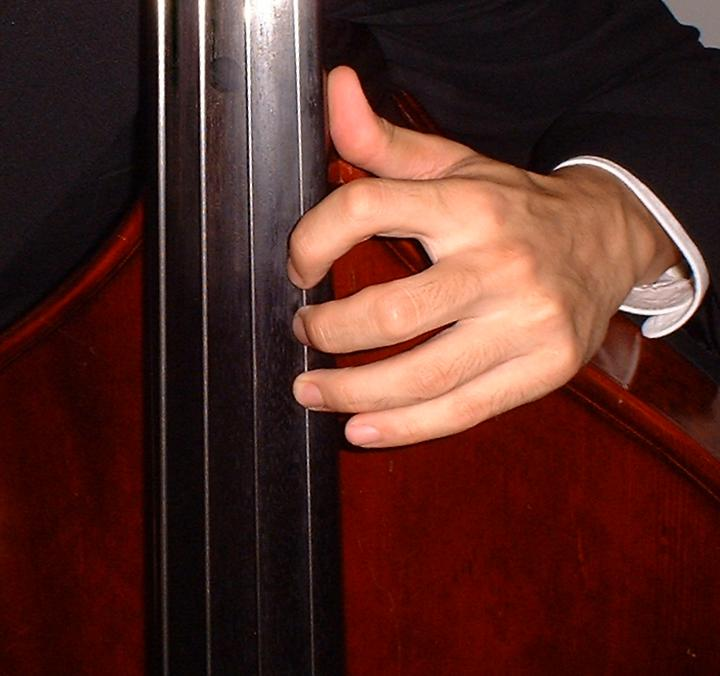
\includegraphics[width=3.75cm]{../Vol1/Pics/Position/6th_1.epsi}\\
{\small 図\thefigure : 第VIポジション\\}
\end{center}
\end{minipage}

\begin{minipage}{260pt}
\subsection{第VIポジションで取れる音}
\begin{music}
\nostartrule
\parindent 0pt
\setclef1{\bass}  
\startpiece
\notes\enotes
\Notes\zchar{20}{G線}\zchar{15}{\bf 1}\wh{f}\zchar{15}{\bf 2}\wh{^f}\zchar{16}{\bf 3}\wh{g}\enotes
\doublebar
\Notes\zchar{15}{\bf 1}\wh{f}\zchar{16}{\bf 2}\wh{_g}\zchar{16}{\bf 3}\wh{=g}\enotes
\doublebar
\Notes\zchar{20}{D線}\zchar{12}{\bf 1}\wh{c}\zchar{12}{\bf 2}\wh{^c}\zchar{13}{\bf 3}\wh{d}\enotes
\doublebar
\Notes\zchar{12}{\bf 1}\wh{c}\zchar{13}{\bf 2}\wh{_d}\zchar{13}{\bf 3}\wh{=d}\enotes
\setdoublebar
\endpiece
\startpiece
\notes\enotes
\Notes\zchar{14}{A線}\zchar{9}{\bf 1}\wh{'G}\zchar{9}{\bf 2}\wh{^G}\zchar{9}{\bf 3}\wh{!a}\enotes
\doublebar
\Notes\zchar{10}{\bf 1}\wh{'G}\zchar{10}{\bf 2}\wh{!_a}\zchar{10}{\bf 3}\wh{=a}\enotes
\doublebar
\Notes\zchar{14}{E線}\zchar{9}{\bf 1}\wh{'D}\zchar{9}{\bf 2}\wh{^D}\zchar{9}{\bf 3}\wh{E}\enotes
\doublebar
\Notes\zchar{9}{\bf 1}\wh{'D}\zchar{9}{\bf 2}\wh{_E}\zchar{9}{\bf 3}\wh{=E}\enotes
\setdoublebar
\endpiece
\end{music}
\end{minipage}
\hfill
\begin{minipage}{140pt}
\addtocounter{figure}{1}
\begin{center}
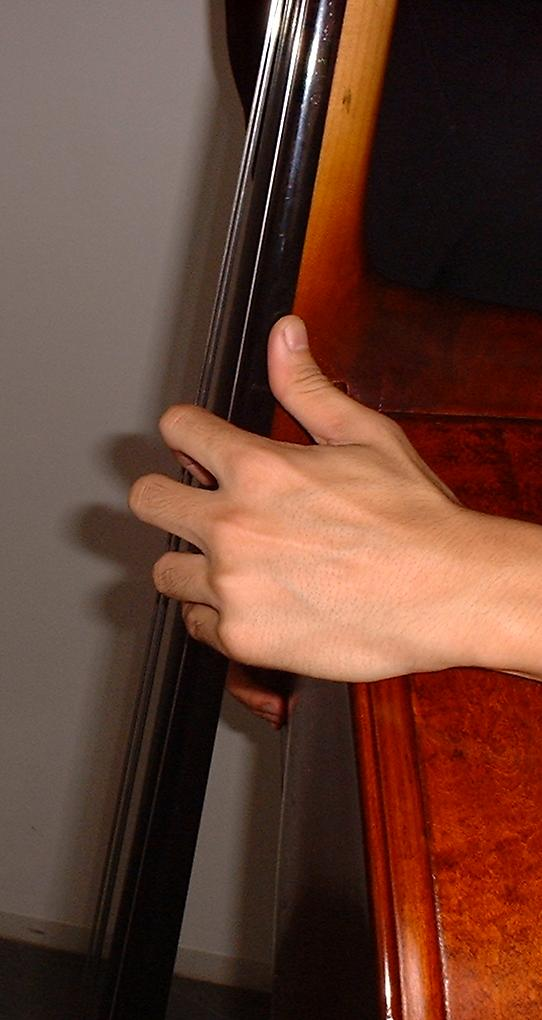
\includegraphics[width=3.75cm]{../Vol1/Pics/Position/6th_2.epsi}\\
{\small 図\thefigure : 親指を指板の横に\\}
\end{center}
\end{minipage}
\end{flushleft}

\subsection{音階練習 \label{6th_scale}}

\begin{music}
\nostartrule
\parindent 0pt
\setclef1{\bass}  
\generalsignature{-2}    
\startpiece
\notes\zchar{14}{変ロ長調(B-dur)音階}\enotes
\Notes\zchar{8}{\bf 1}\qu{'B}\enotes
\notes\ibu{0}{'C}{3}\islurd{0}{C}\qb{0}{C}\tbu{0}\tslur{0}{D}\qb{0}{D}\enotes
\notes\ibl{0}{'E}{3}\qb{0}{E}\qb{0}{F}\qb{0}{G}\tbl{0}\qb{0}{!a}\enotes
\bar
\notes\ibl{0}{b}{0}\isluru{0}{b}\qb{0}{b}\tslur{0}{a}\qb{0}{a}\qb{0}{b}\tbl{0}\zchar{12}{\bf 1}\qb{0}{c}\enotes
\notes\ibl{0}{d}{0}\isluru{0}{d}\qb{0}{d}\tslur{0}{c}\qb{0}{c}\zchar{13}{\bf 2}\qb{0}{d}\tbl{0}\qb{0}{e}\enotes
\bar
\notes\ibl{0}{f}{-1}\isluru{0}{f}\zchar{16}{\bf 1}\qb{0}{f}\tslur{0}{g}\qb{0}{g}\qb{0}{f}\tbl{0}\zchar{14}{\bf 4}\qb{0}{e}\enotes
\notes\ibl{0}{d}{-1}\isluru{0}{d}\qb{0}{d}\tslur{0}{e}\qb{0}{e}\qb{0}{d}\tbl{0}\zchar{12}{\bf 4}\qb{0}{c}\enotes
\bar
\notes\ibl{0}{b}{-3}\qb{0}{b}\zchar{10}{\bf 2}\qb{0}{a}\qb{0}{'G}\tbl{0}\qb{0}{F}\enotes
\notes\ibu{0}{'E}{-3}\qb{0}{E}\qb{0}{D}\qb{0}{C}\tbu{0}\qb{0}{B}\enotes
\endpiece

\generalsignature{-2}    
\startpiece
\notes\zchar{14}{ト短調(g-moll)音階}\enotes
\Notes\zchar{8}{\bf 4}\qu{G}\enotes
\notes\ibu{0}{'A}{3}\islurd{0}{A}\qb{0}{A}\tbu{0}\tslur{0}{B}\qb{0}{B}\enotes
\notes\ibl{0}{'C}{3}\qb{0}{C}\qb{0}{D}\zchar{8}{\bf 1}\qb{0}{=E}\tbl{0}\qb{0}{^F}\enotes
\bar
\Notes\ql{'G}\enotes
\notes\ibl{0}{a}{3}\isluru{0}{a}\qb{0}{a}\tbl{0}\tslur{0}{b}\zchar{11}{\bf 1}\qb{0}{b}\enotes
\notes\ibl{0}{c}{3}\qb{0}{c}\zchar{13}{\bf 1}\qb{0}{d}\qb{0}{=e}\tbl{0}\zchar{15}{\bf 2}\qb{0}{^f}\enotes
\bar
\Notes\ql{g}\enotes
\notes\ibl{0}{f}{-2}\isluru{0}{f}\qb{0}{=f}\tbl{0}\tslur{0}{e}\zchar{14}{\bf 4}\qb{0}{_e}\enotes
\notes\ibl{0}{d}{-3}\qb{0}{d}\zchar{12}{\bf 4}\qb{0}{c}\qb{0}{b}\tbl{0}\zchar{10}{\bf 2}\qb{0}{a}\enotes
\bar
\notes\ibl{0}{'G}{-3}\qb{0}{G}\qb{0}{F}\qb{0}{E}\tbl{0}\qb{0}{D}\enotes
\notes\ibu{0}{'C}{-3}\qb{0}{C}\qb{0}{B}\qb{0}{A}\tbu{0}\qb{0}{!G}\enotes
\endpiece

\generalsignature{1}    
\startpiece
\notes\zchar{14}{ト長調(G-dur)音階}\enotes
\Notes\zchar{8}{\bf 2}\qu{G}\enotes
\notes\ibu{0}{'A}{3}\islurd{0}{A}\qb{0}{A}\tbu{0}\tslur{0}{B}\qb{0}{B}\enotes
\notes\ibl{0}{'C}{3}\qb{0}{C}\qb{0}{D}\qb{0}{E}\tbl{0}\qb{0}{F}\enotes
\bar
\Notes\ql{'G}\enotes
\notes\ibl{0}{a}{3}\isluru{0}{a}\qb{0}{a}\tbl{0}\tslur{0}{b}\zchar{12}{\bf 2}\qb{0}{b}\enotes
\notes\ibl{0}{c}{3}\qb{0}{c}\zchar{13}{\bf 1}\qb{0}{d}\qb{0}{e}\tbl{0}\zchar{15}{\bf 2}\qb{0}{f}\enotes
\bar
\Notes\ql{g}\enotes
\notes\ibl{0}{f}{-2}\isluru{0}{f}\qb{0}{f}\tbl{0}\tslur{0}{e}\zchar{15}{\bf 4}\qb{0}{e}\enotes
\notes\ibl{0}{d}{-3}\qb{0}{d}\zchar{12}{\bf 4}\qb{0}{c}\qb{0}{b}\tbl{0}\zchar{10}{\bf 1}\qb{0}{a}\enotes
\bar
\notes\ibl{0}{'G}{-3}\qb{0}{G}\qb{0}{F}\qb{0}{E}\tbl{0}\qb{0}{D}\enotes
\notes\ibu{0}{'C}{-3}\qb{0}{C}\qb{0}{B}\qb{0}{A}\tbu{0}\qb{0}{!G}\enotes
\endpiece

\generalsignature{2}    
\startpiece
\notes\zchar{14}{ロ短調(h-moll)音階}\enotes
\Notes\zchar{8}{\bf 1}\qu{'B}\enotes
\notes\ibu{0}{'C}{3}\islurd{0}{C}\qb{0}{C}\tbu{0}\tslur{0}{D}\qb{0}{D}\enotes
\notes\ibl{0}{'E}{3}\qb{0}{E}\qb{0}{F}\zchar{10}{\bf 1}\qb{0}{^G}\tbl{0}\zchar{11}{\bf 2}\qb{0}{!^a}\enotes
\bar
\notes\ibl{0}{b}{0}\isluru{0}{b}\qb{0}{b}\tslur{0}{a}\qb{0}{^a}\qb{0}{b}\tbl{0}\zchar{12}{\bf 2}\qb{0}{c}\enotes
\notes\ibl{0}{d}{0}\isluru{0}{d}\qb{0}{d}\tslur{0}{c}\qb{0}{c}\zchar{13}{\bf 1}\qb{0}{d}\tbl{0}\qb{0}{e}\enotes
\bar
\notes\ibl{0}{f}{-1}\isluru{0}{f}\zchar{16}{\bf 2}\qb{0}{f}\tslur{0}{g}\qb{0}{g}\qb{0}{f}\tbl{0}\zchar{14}{\bf 4}\qb{0}{e}\enotes
\notes\ibl{0}{d}{-1}\isluru{0}{d}\qb{0}{d}\tslur{0}{e}\qb{0}{e}\qb{0}{d}\tbl{0}\zchar{12}{\bf 4}\qb{0}{c}\enotes
\bar
\notes\ibl{0}{b}{-3}\qb{0}{b}\zchar{10}{\bf 1}\qb{0}{=a}\qb{0}{'=G}\tbl{0}\qb{0}{F}\enotes
\notes\ibu{0}{'E}{-3}\qb{0}{E}\qb{0}{D}\qb{0}{C}\tbu{0}\qb{0}{B}\enotes
\endpiece
\end{music}

\subsection{第VIポジションで弾ける名曲}
\documentclass{jarticle}
\usepackage{musixdoc}
\startmuflex\makeindex

\begin{document}

\subsubsection*{�٥�ꥪ����: ���۸���� ��4�ھϡ���Ƭ��ؤιԿʡפ��}

\begin{music}
\nostartrule
\setclef1{\bass}
\generalsignature{-2}    
\generalmeter{\allabreve}
\parindent 0pt
\startbarno=17
\def\writebarno{\tenrm\the\barno\barnoadd}
\def\raisebarno{2\internote}
\def\shiftbarno{0.1\Interligne}
\systemnumbers
\startpiece\bigaccid
\notes\zchar{24}{\bf Allegretto non troppo (\metron{\hu}{72})}\enotes
\Notes\zchar{-8}{\f}\zchar{-4}{VI}\zchar{12}{\downbow}\zchar{9}{\bf 1}\ql{'G}\qp\zchar{-4}{\ff}\zchar{19}{\upbow}\zchar{16}{\bf 3}\hl{!g}\enotes
\bar
\Notes\zchar{-3}{\icresc}\isluru{0}{f}\zchar{17}{\downbow}\zchar{15}{\bf 1}\hl{f}\zchar{-3}{\tdecresc}\tslur{0}{e}\zchar{-5}{\small [}\roffset{0.55}{\zchar{-4}{\small III}}\roffset{0.55}{\zchar{-7}{\small IV}}\zchar{14}{\bf 4}\ql{e}\enotes
\notes\zchar{-7}{\it dim.}\ibl{0}{d}{-2}\zchar{13}{\upbow}\upz{d}\qb{0}{d}\tbl{0}\zchar{-4}{II}\zchar{15}{\downbow}\zchar{13}{\bf 4}\upz{c}\qb{0}{c}\enotes
\bar
\Notes\zchar{12}{\upbow}\ql{b}\qp\zchar{14}{\upbow}\zchar{-4}{I}\zchar{11}{\bf 1}\ql{a}\qp\enotes
\bar
\Notes\zchar{11}{\icresc}\isluru{0}{'G}\zchar{-4}{II}\zchar{15}{\downbow}\zchar{13}{\bf 4}\hl{G}\zchar{11}{\tdecresc}\tslur{0}{F}\ql{F}\enotes
\notes\ibl{0}{'E}{-2}\loffset{0.7}{\zchar{-7}{\small [}}\roffset{0.3}{\zchar{-6}{\small II}}\zchar{-9}{\small III}\zchar{12}{\upbow}\zchar{9}{\bf 4}\upz{E}\qb{0}{E}\tbl{0}\zchar{9}{\downbow}\upz{D}\qb{0}{D}\enotes
\bar
\Notes\zchar{-4}{half}\zchar{14}{\upbow}\zchar{11}{\bf 4}\qu{'C}\qp\zchar{10}{\upbow}\qu{B}\qp\enotes
\bar
\Notes\zchar{11}{\icresc}\islurd{0}{'A}\zchar{-5}{II}\zchar{14}{\downbow}\zchar{12}{\bf 4}\hu{A}\zchar{11}{\tdecresc}\tslur{0}{!G}\qu{!G}\enotes
\notes\ibu{0}{'A}{2}\loffset{0.7}{\zchar{-5}{\small [}}\roffset{0.3}{\zchar{-4}{\small II}}\zchar{-7}{\small III}\zchar{12}{\upbow}\zchar{9}{\bf 2}\qb{0}{A}\tbu{0}\zchar{12}{\downbow}\zchar{9}{\bf 4}\qb{0}{B}\enotes
\bar
\Notes\zchar{-7}{\p}\zchar{-4}{II}\zchar{12}{\upbow}\zchar{9}{\bf 1}\qu{'C}\qp\zchar{12}{\upbow}\zchar{9}{\bf 4}\qu{A}\qp\enotes
\bar
\Notes\zchar{8}{\downbow}\hl{'D}\hp\enotes
\bar
\Notes\zchar{-7}{\mf}\zchar{-4}{VI}\zchar{11}{\downbow}\zchar{9}{\bf 1}\ql{'G}\qp\zchar{-4}{\f}\zchar{18}{\upbow}\zchar{15}{\bf 3}\hl{!g}\enotes
\bar
\Notes\zchar{-3}{\icresc}\isluru{0}{f}\zchar{17}{\downbow}\zchar{15}{\bf 1}\hl{f}\zchar{-3}{\tdecresc}\tslur{0}{e}\zchar{-5}{\small [}\roffset{0.55}{\zchar{-4}{\small III}}\roffset{0.55}{\zchar{-7}{\small IV}}\zchar{14}{\bf 4}\ql{e}\enotes
\notes\ibl{0}{d}{-2}\zchar{14}{\upbow}\upz{d}\qb{0}{d}\tbl{0}\zchar{-4}{II}\zchar{16}{\downbow}\zchar{14}{\bf 4}\upz{d}\qb{0}{c}\enotes
\bar
\Notes\zchar{-4}{\it dim.}\zchar{11}{\upbow}\ql{b}\qp\zchar{-4}{I}\zchar{14}{\upbow}\zchar{11}{\bf 1}\ql{a}\qp\enotes
\bar
\Notes\zchar{-6}{\icresc}\isluru{0}{'G}\zchar{-4}{II}\zchar{12}{\downbow}\zchar{10}{\bf 4}\hl{G}\zchar{-6}{\tdecresc}\tslur{0}{F}\ql{F}\enotes
\notes\ibl{0}{'E}{-2}\loffset{0.7}{\zchar{-7}{\small [}}\roffset{0.3}{\zchar{-6}{\small II}}\zchar{-9}{\small III}\zchar{9}{\bf 4}\zchar{12}{\upbow}\upz{E}\qb{0}{E}\tbl{0}\zchar{9}{\downbow}\upz{D}\qb{0}{D}\enotes
\bar
\Notes\zchar{-4}{half}\zchar{13}{\upbow}\zchar{10}{\bf 4}\lpz{'C}\qu{C}\qp\zchar{10}{\upbow}\lpz{B}\qu{B}\qp\enotes
\bar
\Notes\zchar{-7}{\p \decrescendo{6mm}}\islurd{0}{'A}\zchar{-4}{II}\zchar{12}{\downbow}\zchar{10}{\bf 4}\hu{A}\tslur{0}{!G}\qu{G}\enotes
\notes\ibu{0}{'A}{2}\loffset{0.7}{\zchar{-5}{\small [}}\roffset{0.3}{\zchar{-4}{\small II}}\zchar{-7}{\small III}\zchar{13}{\upbow}\zchar{10}{\bf 2}\qb{0}{A}\tbu{0}\zchar{11}{\downbow}\qb{0}{B}\enotes
\bar
\Notes\zchar{-4}{half}\zchar{13}{\upbow}\zchar{10}{\bf 4}\qu{'C}\qp\zchar{-4}{\pp}\zchar{10}{\upbow}\qu{B}\qp\enotes
\bar
\Notes\zchar{9}{\downbow}\hl{'E}\hp\enotes
\mulooseness=0
\setdoublebar\endpiece
\end{music}

\endmuflex
\end{document}

\documentclass{jarticle}
\usepackage{musixdoc}
\startmuflex\makeindex

\begin{document}

\subsubsection*{���㥤���ե�����: ���۽��ʡ֥��ᥪ�ȥ���ꥨ�åȡפ��}

\begin{music}
\setclef1{\bass}
\generalsignature{2}    
\generalmeter{\meterC}
\parindent 0pt
\nostartrule
\startpiece\bigaccid
\qspace
\notes\zchar{15}{\bf (Allegro giusto)}\enotes
\Notes\hpause\zchar{-5}{\mf}\zchar{8}{\upbow}\cl{'D}\ds\isluru{0}{!a}\zchar{10}{\downbow}\ql{a}\enotes
\bar
\Notes\ibl{0}{'D}{0}\tslur{0}{!a}\qb{0}{a}\qb{0}{'D}\qb{0}{D}\tbl{0}\qb{0}{E}\enotes
\NOtes\ibl{0}{'F}{-1}\zchar{8}{\downbow}\qbp{0}{F}\enotes
\notes\tbbl{0}\tbl{0}\zchar{8}{\downbow}\qb{0}{'E}\enotes
\Notes\zchar{8}{\upbow}\cl{'D}\ds\enotes
\bar
\Notes\ds\zchar{8}{\upbow}\cl{'D}\enotes
\Notes\ibl{0}{'D}{2}\qb{0}{D}\tbl{0}\qb{0}{=F}\enotes
\NOtes\ibl{0}{'G}{-1}\zchar{8}{\downbow}\qbp{0}{G}\enotes
\notes\tbbl{0}\tbl{0}\zchar{8}{\downbow}\qb{0}{'F}\enotes
\Notes\zchar{8}{\upbow}\cl{'E}\ds\enotes
\bar
\Notes\ds\zchar{14}{\upbow}\cl{d}\enotes
\NOtes\ibl{0}{c}{-1}\zchar{13}{\downbow}\qbp{0}{c}\enotes
\notes\tbbl{0}\tbl{0}\zchar{10}{\upbow}\qb{0}{a}\enotes
\Notes\zchar{14}{\downbow}\cl{d}\ds\qp\enotes
\alaligne
\qspace
\Notes\hpause\zchar{8}{\upbow}\cl{'G}\ds\isluru{0}{!d}\zchar{14}{\downbow}\ql{d}\enotes
\bar
\Notes\ibl{0}{'G}{0}\tslur{0}{!d}\qb{0}{d}\qb{0}{'G}\qb{0}{G}\tbl{0}\qb{0}{!a}\enotes
\NOtes\ibl{0}{b}{-1}\zchar{10}{\downbow}\qbp{0}{_b}\enotes
\notes\tbbl{0}\tbl{0}\zchar{10}{\downbow}\qb{0}{a}\enotes
\Notes\zchar{8}{\upbow}\cl{'G}\ds\enotes
\bar
\Notes\ds\zchar{8}{\upbow}\cl{'G}\enotes
\Notes\ibl{0}{'G}{2}\qb{0}{G}\tbl{0}\qb{0}{!_b}\enotes
\NOtes\ibl{0}{c}{-1}\zchar{11}{\downbow}\qbp{0}{=c}\enotes
\notes\tbbl{0}\tbl{0}\zchar{10}{\downbow}\qb{0}{b}\enotes
\Notes\zchar{9}{\upbow}\cl{a}\ds\enotes
\bar
\Notes\ds\zchar{-4}{VI}\zchar{18}{\upbow}\zchar{16}{\bf 3}\cl{g}\enotes
\NOtes\ibl{0}{d}{-1}\zchar{16}{\downbow}\zchar{14}{\bf 2}\qbp{0}{f}\enotes
\notes\tbbl{0}\tbl{0}\zchar{15}{\upbow}\zchar{12}{\bf 3}\qb{0}{d}\enotes
\Notes\zchar{18}{\downbow}\zchar{16}{\bf 3}\cl{g}\ds\qp\enotes
\setdoublebar
\endpiece
\end{music}

\endmuflex
\end{document}

\documentclass{jarticle}
\usepackage{musixdoc}
\startmuflex\makeindex

\begin{document}
\subsubsection*{�ϥ��ɥ�: �������45�� �Ť�ûĴ �ֹ��̡� ��4�ھϤ��}
\begin{music}
\nostartrule
\setclef1{\bass}
\generalsignature{3}    
\generalmeter{\meterfrac38}
\parindent 0pt
\startbarno=55
\def\writebarno{\tenrm\the\barno\barnoadd}
\def\raisebarno{2\internote}
\def\shiftbarno{0.1\Interligne}
\systemnumbers
\startpiece\bigaccid
\notes\zchar{15}{\bf Adagio}\zchar{-6}{\p}\enotes
\notes\ibbl{0}{'C}{4}\zchar{-8}{III}\zchar{10}{\downbow}\zchar{8}{\bf 1}\qb{0}{A!a}\tbl{0}\tbbl{0}\qb{0}{!a}\enotes
\notes\ibbl{0}{c}{0}\qb{0}{ca}\tbl{0}\tbbl{0}\qb{0}{a}\enotes
\notes\ibbl{0}{c}{0}\qb{0}{da}\tbl{0}\tbbl{0}\qb{0}{a}\enotes
\bar
\notes\ibbl{0}{c}{0}\zchar{11}{\upbow}\qb{0}{ca}\tbl{0}\tbbl{0}\qb{0}{a}\enotes
\notes\ibbl{0}{c}{0}\qb{0}{aa}\tbl{0}\tbbl{0}\qb{0}{a}\enotes
\notes\ibbl{0}{c}{0}\loffset{0.7}{\zchar{-4}{\small [}}\roffset{0.3}{\zchar{-3}{\small V}}\zchar{-6}{\small VI}\zchar{15}{\bf 4}\qb{0}{f}\zchar{10}{\bf 1}\qb{0}{a}\tbl{0}\tbbl{0}\qb{0}{a}\enotes
\bar
\notes\ibbl{0}{c}{0}\zchar{14}{\downbow}\qb{0}{ea}\tbl{0}\tbbl{0}\qb{0}{a}\enotes
\notes\ibbl{0}{c}{0}\qb{0}{aa}\tbl{0}\tbbl{0}\qb{0}{a}\enotes
\notes\ibbl{0}{c}{0}\qb{0}{da}\tbl{0}\tbbl{0}\qb{0}{a}\enotes
\bar
\notes\ibbl{0}{c}{0}\zchar{-4}{III}\zchar{15}{\upbow}\zchar{12}{\bf 2}\qb{0}{ca}\tbl{0}\tbbl{0}\qb{0}{a}\enotes
\notes\ibbl{0}{c}{0}\qb{0}{aa}\tbl{0}\tbbl{0}\qb{0}{a}\enotes
\notes\ibbl{0}{e}{-5}\loffset{0.7}{\zchar{-4}{\small [}}\roffset{0.3}{\zchar{-3}{\small V}}\zchar{-6}{\small VI}\zchar{14}{\bf 1}\qb{0}{ec}\tbl{0}\tbbl{0}\zchar{-4}{V}\zchar{10}{\bf 1}\qb{0}{^a}\enotes
\bar
\notes\ibbl{0}{c}{0}\zchar{11}{\downbow}\qb{0}{bb}\tbl{0}\tbbl{0}\qb{0}{b}\enotes
\notes\ibbl{0}{c}{0}\qb{0}{bb}\tbl{0}\tbbl{0}\qb{0}{b}\enotes
\notes\ibbl{0}{c}{0}\loffset{1}{\zchar{-4}{VI}}\zchar{16}{\bf 3}\qb{0}{=g}\loffset{0.7}{\zchar{-4}{\small [}}\roffset{0.3}{\zchar{-3}{\small V}}\zchar{-6}{\small VI}\zchar{11}{\bf 1}\qb{0}{b}\tbl{0}\tbbl{0}\qb{0}{b}\enotes
\bar
\notes\ibbl{0}{c}{0}\zchar{15}{\upbow}\qb{0}{fb}\tbl{0}\tbbl{0}\qb{0}{b}\enotes
\notes\ibbl{0}{c}{0}\qb{0}{bb}\tbl{0}\tbbl{0}\qb{0}{b}\enotes
\notes\ibbl{0}{c}{0}\zchar{-4}{IV}\zchar{14}{\bf 4}\qb{0}{eb}\tbl{0}\tbbl{0}\qb{0}{b}\enotes
\bar
\notes\ibbl{0}{c}{0}\zchar{13}{\downbow}\qb{0}{db}\tbl{0}\tbbl{0}\qb{0}{b}\enotes
\notes\ibbl{0}{c}{0}\qb{0}{bb}\tbl{0}\tbbl{0}\qb{0}{b}\enotes
\notes\ibbl{0}{f}{-5}\loffset{0.7}{\zchar{-4}{\small [}}\roffset{0.3}{\zchar{-3}{\small V}}\zchar{-6}{\small VI}\zchar{15}{\bf 4}\qb{0}{f}\zchar{-4}{V}\zchar{13}{\bf 1}\qb{0}{^d}\tbl{0}\tbbl{0}\loffset{0.7}{\zchar{-4}{\small [}}\roffset{0.3}{\zchar{-3}{\small V}}\zchar{-6}{\small VI}\zchar{12}{\bf 2}\qb{0}{^b}\enotes
\bar
\notes\ibbl{0}{e}{0}\zchar{15}{\upbow}\zchar{12}{\bf 4}\qb{0}{cc}\tbl{0}\tbbl{0}\qb{0}{c}\enotes
\notes\ibbl{0}{e}{0}\zchar{14}{\bf 2}\qb{0}{^ec}\tbl{0}\tbbl{0}\qb{0}{c}\enotes
\notes\ibbl{0}{'E}{3}\qb{0}{C!c}\tbl{0}\tbbl{0}\qb{0}{!c}\enotes
\bar
\notes\ibbl{0}{'E}{3}\zchar{10}{\downbow}\qb{0}{C!c}\tbl{0}\tbbl{0}\qb{0}{!c}\enotes
\notes\ibbl{0}{e}{0}\qb{0}{^ec}\tbl{0}\tbbl{0}\qb{0}{c}\enotes
\notes\ibbl{0}{'E}{3}\qb{0}{C!c}\tbl{0}\tbbl{0}\qb{0}{!c}\enotes
\bar
\notes\ibbl{0}{'E}{3}\zchar{10}{\upbow}\qb{0}{C!c}\tbl{0}\tbbl{0}\qb{0}{!c}\enotes
\notes\ibbl{0}{e}{0}\qb{0}{^ec}\tbl{0}\tbbl{0}\qb{0}{c}\enotes
\notes\ibbl{0}{'E}{3}\qb{0}{C!c}\tbl{0}\tbbl{0}\qb{0}{!c}\enotes
\bar
\notes\ibbl{0}{'E}{3}\zchar{10}{\downbow}\qb{0}{C!c}\tbl{0}\tbbl{0}\qb{0}{!c}\enotes
\notes\ibbl{0}{e}{0}\qb{0}{^ec}\tbl{0}\tbbl{0}\qb{0}{c}\enotes
\notes\ibbl{0}{'E}{3}\qb{0}{C!c}\tbl{0}\tbbl{0}\qb{0}{!c}\enotes
\bar
\notes\ibbl{0}{'E}{4}\zchar{10}{\upbow}\qb{0}{C!c}\tbl{0}\tbbl{0}\qb{0}{!c}\enotes
\notes\ibbl{0}{a}{4}\qb{0}{'G!c}\tbl{0}\tbbl{0}\qb{0}{!c}\enotes
\notes\ibbl{0}{'F}{3}\qb{0}{^EG}\tbl{0}\tbbl{0}\qb{0}{G}\enotes
\bar
\Notes\zchar{10}{\downbow}\cu{'C}\ds\ds\enotes
\mulooseness=0
\setdoublebar\endpiece
\end{music}

\endmuflex
\end{document}

